	% HMC Math dept HW template example
	% v0.04 by Eric J. Malm, 10 Mar 2005
	\documentclass[10pt,a4paper,boxed]{hmcpset}

	% set 1-inch margins in the document
	% \usepackage[margin=1in]{geometry}
	\usepackage{enumerate}
	\usepackage{tikz}
	\usetikzlibrary{positioning}
	\usepackage{pgfplots}
	\usepackage{amsmath}
	\usepackage{amsfonts}
	\usepackage{amssymb}

	% include this if you want to import graphics files with /includegraphics
	\usepackage{graphicx}

	\renewcommand*{\familydefault}{\sfdefault}
	\newcommand{\vect}[1]{\mathbf{#1}}
	\DeclareMathOperator{\gain}{Gain}
	\DeclareMathOperator{\entropy}{H}
	\DeclareMathOperator{\prob}{P}

	\tikzset{node distance=2cm, inner/.style={draw,circle}, leaf/.style={draw,rectangle}}

	% info for header block in upper right hand corner
	\name{Group 6: Timm Behner, Philipp Bruckschen, Patrick Kaster, Markus Schwalb}
	\class{MA-INF 4111 - Intelligent Learning and Analysis Systems: Machine Learning}
	\assignment{Exercise Sheet 2}
	% \duedate{09/03/2004}

	\begin{document}

	\begin{problem}[1. TDIDT]
	\end{problem}
	\begin{solution}
	Begin with the emtpy decision tree and search for the best split in all
	attributes.

	Entropy of examples $\entropy(X) = 0.994$
	\begin{description}
		\item[Wind]\hfill

			\begin{tabular}[H]{l|ll}
				& + & - \\ \hline
				Weak & 3 & 2 \\
				Strong & 3 & 3 \\
			\end{tabular}
			\begin{align}
				\gain(X|\mathrm{Wind}) &= \entropy(X) - \sum_{w \in \left\{ \mathrm{Weak}, \neg\mathrm{Weak}  \right\} } \prob(\mathrm{Wind}=w) \entropy(X|\mathrm{Wind}=w) \\
															 &= 0.0072
			\end{align}

		\item[Temperature] \hfill \\
			Compute the best splitting test for this attribute\\
				\begin{tabular}[H]{ll}
					Value & Outcome \\
					7&+\\
					8&+\\
					10&+\\
					11&+\\
					20&+\\
					21&-\\
					23&+\\
					23&-\\
					31&-\\
					32&-\\
					34&-\\
				\end{tabular}

			\begin{tabular}[H]{l|ll}
				& + & - \\ \hline
				$20.5 > $		& 5 & 0 \\
				$20.5 \leq$ & 1 & 5 \\
			\end{tabular}
			$\entropy(X|\mathrm{Temp}<20.5) = 0$
			$\entropy(X|\mathrm{Temp}\geq 20.5) = 0.65$

			\begin{tabular}[H]{l|ll}
				& + & - \\ \hline
				$22 > $		& 5 & 1 \\
				$22 \leq$ & 1 & 4 \\
			\end{tabular}
			$\entropy(X|\mathrm{Temp}<22) = 0.65$
			$\entropy(X|\mathrm{Temp}\geq 22) = 0.7219$

			From this follows that the maximum gain for this attribute is 
			$\gain(X|\mathrm{Temp} \leq 20.5) = 0.6395$

		\item[Outlook]  \hfill \\
			\begin{tabular}[H]{l|ll}
				& + & - \\ \hline
				Sunny				 & 2 & 2 \\
				$\neg$ Sunny & 4 & 3 \\
			\end{tabular}
			$\Rightarrow \gain(X|\mathrm{Outlook}=\mathrm{Sunny}) = 0.0034$

			\begin{tabular}[H]{l|ll}
				& + & - \\ \hline
				Overcast				 & 1 & 2 \\
				$\neg$ Overcast & 5 & 3 \\
			\end{tabular}
			$\Rightarrow \gain(X|\mathrm{Outlook}=\mathrm{Overcast}) = 0.0494$

			\begin{tabular}[H]{l|ll}
				& + & - \\ \hline
				Rain				 & 3 & 1 \\
				$\neg$ Rain & 3 & 4 \\
			\end{tabular}
			$\Rightarrow \gain(X|\mathrm{Outlook}=\mathrm{Rain}) = 0.072$

			Now check for 
			\begin{align}
				\gain(X|\mathrm{Outlook}\in \left\{ \mathrm{Rain},\mathrm{Overcast} \right\} = 0.0035
			\end{align}
			From this follows that the maximum information gain for this attribute is 
			$\Rightarrow \gain(X|\mathrm{Outlook}=\mathrm{Rain}) = 0.072$
			\end{description}
			The attribute with the maximum information gain is Temperatur (split with $20.5\leq$)\\[2em]
			\begin{center}
				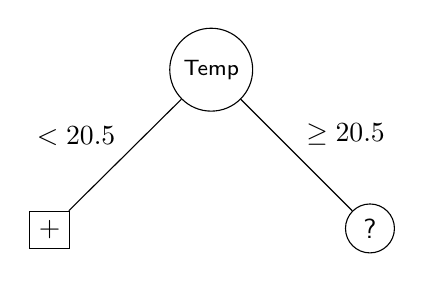
\begin{tikzpicture}
					\node[inner] (T) {\footnotesize Temp};
					\node[inner] (Tn) [below right=of T] {?};

					\node[leaf] (L1) [below left=of T] {+};

					\path[draw]
					(T) -- node[above left] {$<20.5$} (L1)
					(T) -- node[above right] {$\geq 20.5$} (Tn);
				\end{tikzpicture}
			\end{center}

			Search for best attribute to split in $\left\{ \mathrm{Overcast},\mathrm{Wind} \right\}$	
			\begin{description}
				\item[Overcast] \hfill \\
				\begin{tabular}[H]{l|ll}
					& + & - \\ \hline
					Sunny				 & 1 & 2 \\
					$\neg$ Sunny & 0 & 3 \\
				\end{tabular}
				$\Rightarrow \gain(X|\mathrm{Outlook}=\mathrm{Sunny}) = 0.1901$

				\begin{tabular}[H]{l|ll}
					& + & - \\ \hline
					Overcast				 & 0 & 2 \\
					$\neg$ Overcast & 1 & 3 \\
				\end{tabular}
				$\Rightarrow \gain(X|\mathrm{Outlook}=\mathrm{Overcast}) = 0.1091$

				\begin{tabular}[H]{l|ll}
					& + & - \\ \hline
					Rain				 & 0 & 1 \\
					$\neg$ Rain & 1 & 4 \\
				\end{tabular}
				$\Rightarrow \gain(X|\mathrm{Outlook}=\mathrm{Rain}) = 0.0484$

				And $\gain(X|\mathrm{Outlook} \in \left\{ \mathrm{Sunny}, \mathrm{Overcast} \right\}) = 0.0484$

			\item[Wind] \hfill \\
				\begin{tabular}[H]{l|ll}
					& + & - \\ \hline
					Weak				 & 1 & 4 \\
					$\neg$ Weak & 0 & 1 \\
				\end{tabular}
				$\Rightarrow \gain(X|\mathrm{Wind}) = 0.1091$

		\end{description}

		From this follows that the maximum information gain for this node is
		$\gain(X|\mathrm{Outlook} = \mathrm{Sunny}) = 0.1909$
			\begin{center}
			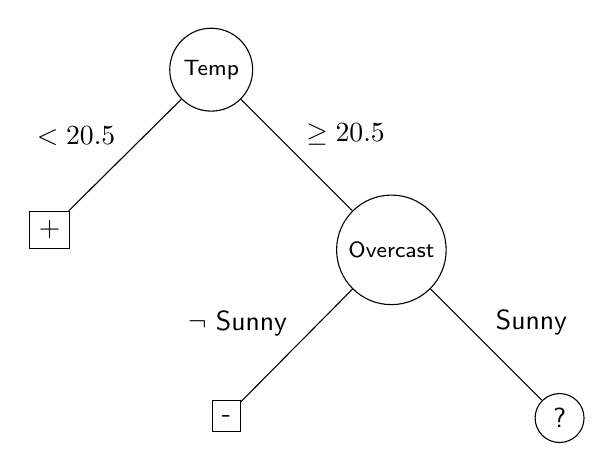
\begin{tikzpicture}
				\node[inner] (T) {\footnotesize Temp};
				\node[inner] (O) [below right=of T] {\footnotesize Overcast};
				\node[inner] (Tn) [below right=of O] {?};

				\node[leaf] (L1) [below left=of T] {+};
				\node[leaf] (L2) [below left=of O] {-};

				\path[draw]
				(T) -- node[above left] {$<20.5$} (L1)
				(T) -- node[above right] {$\geq 20.5$} (O)
				(O) -- node[above left] {$\neg$ Sunny } (L2)
				(O) -- node[above right] { Sunny } (Tn);
			\end{tikzpicture}
		\end{center}

		Now only the attribute Wind is left.
		\begin{center}
			\begin{tikzpicture}
				\node[inner] (T) {\footnotesize Temp};
				\node[inner] (O) [below right=of T] {\footnotesize Overcast};
				\node[inner] (W) [below right=of O] {\footnotesize Wind};

				\node[leaf] (L1) [below left=of T] {+};
				\node[leaf] (L2) [below left=of O] {-};
				\node[leaf] (L3) [below left=of W] {-};
				\node[leaf] (L4) [below right=of W] {+};

				\path[draw]
				(T) -- node[above left] {$<20.5$} (L1)
				(T) -- node[above right] {$\geq 20.5$} (O)
				(O) -- node[above left] {$\neg$ Sunny } (L2)
				(O) -- node[above right] { Sunny } (W)
				(W) -- node[above left] { Weak } (L3)
				(W) -- node[above right] {$\neg$ Weak} (L4);
			\end{tikzpicture}
		\end{center}
		where the left right leaf of the Wind node was classified as positive,
		because at least half of the examples in this node were positive.
\end{solution}

%\problemlist{Rudin 3.5, Saff and Snider 1.5.11, 1.7.5ad,\\Dummit and Foote 1.1.25, Logan 1.8.6}
\begin{problem}[2. Decision Tree Representations of Boolean Functions]
\end{problem}
\begin{solution}
	\begin{enumerate}
		\item $f(A,B) = A \vee B$ \hfill \\[1em]
			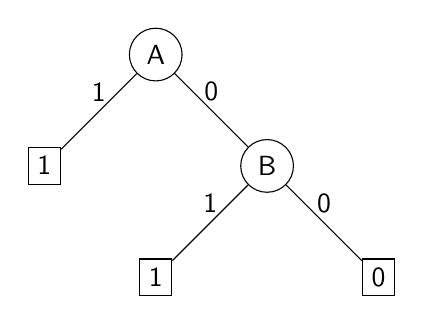
\begin{tikzpicture}
				\node[inner] (A) {A};
				\node[inner] (B) [below right of=A] {B};
				\node[leaf]  (L1) [below left of=A] {1};
				\node[leaf]  (L2) [below left of=B] {1};
				\node[leaf]  (L3) [below right of=B] {0};

				\path[draw]
					(A) -- node[above] {0} (B)
					(A) -- node[above] {1} (L1)
					(B) -- node[above] {1} (L2)
					(B) -- node[above] {0} (L3);
			\end{tikzpicture}

		\item $f(A,B) = A \wedge B$ \hfill \\[1em]
			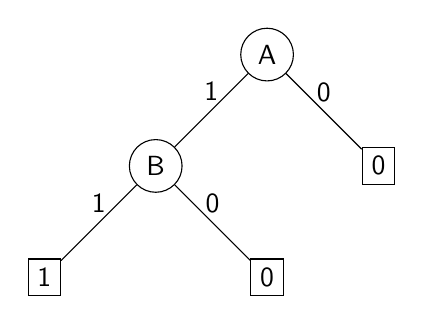
\begin{tikzpicture}
				\node[inner] (A) {A};
				\node[inner] (B) [below left of=A] {B};
				\node[leaf]  (L1) [below right of=A] {0};
				\node[leaf]  (L2) [below left of=B] {1};
				\node[leaf]  (L3) [below right of=B] {0};

				\path[draw]
					(A) -- node[above] {1} (B)
					(A) -- node[above] {0} (L1)
					(B) -- node[above] {1} (L2)
					(B) -- node[above] {0} (L3);
			\end{tikzpicture}

		\item  $f(A,B) = A \oplus B$ \hfill \\[1em]
			\begin{tikzpicture}
				\node[inner] (A) {A};
				\node[inner] (B1) [below left=of A,xshift=-1cm] {B};
				\node[inner] (B2) [below right=of A,xshift=1cm] {B};
				\node[leaf]  (L1) [below left=of B1] {0};
				\node[leaf]  (L2) [below right=of B1] {1};
				\node[leaf]  (L3) [below left=of B2] {1};
				\node[leaf]  (L4) [below right=of B2] {0};

				\path[draw]
				(A) -- node[above] {1} (B1)
				(A) -- node[above] {0} (B2)
				(B1) -- node[above] {1} (L1)
				(B1) -- node[above] {0} (L2)
				(B2) -- node[above] {1} (L3)
				(B2) -- node[above] {0} (L4)
				;

			\end{tikzpicture}

		\item $f(A,B,C,D) = (A \vee B) \wedge (C \vee \neg D \vee E)$ \hfill \\[1em]

			\begin{tikzpicture}
				\node[inner] (A) {A};
				\node[inner] (C1) [below left=of A,xshift=-2cm] {C};
				\node[inner] (B) [below right=of A,xshift=2cm] {B};
				\node[inner] (D1) [below right=of C1,xshift=-0.5cm] {D};
				\node[inner] (E1) [below left=of D1] {E};
				\node[inner] (C2) [below left=of B] {C};
				\node[inner] (D2) [below right=of C2] {D};
				\node[inner] (E2) [below left=of D2] {E};

				\node[leaf] (L1) [below left=of C1] {1};
				\node[leaf] (L2) [below left=of E1] {1};
				\node[leaf] (L3) [below right=of E1] {0};
				\node[leaf] (L4) [below right=of D1] {1};

				\node[leaf] (L5) [below left=of C2] {1};
				\node[leaf] (L6) [below left=of E2] {1};
				\node[leaf] (L7) [below right=of E2] {0};
				\node[leaf] (L8) [below right=of D2] {1};

				\node[leaf] (L9) [below right=of B] {0};

				\path[draw]
				(A) -- node[above] {1} (C1)
				(A) -- node[above] {0} (B)
				(B) -- node[above] {1} (C2)
				(B) -- node[above] {0} (L9)

				(C1) -- node[above] {1} (L1)
				(C1) -- node[above] {0} (D1)
				(D1) -- node[above] {0} (L4)
				(D1) -- node[above] {1} (E1)
				(E1) -- node[above] {1} (L2)
				(E1) -- node[above] {0} (L3)

				(C2) -- node[above] {1} (L5)
				(C2) -- node[above] {0} (D2)
				(D2) -- node[above] {0} (L8)
				(D2) -- node[above] {1} (E2)
				(E2) -- node[above] {1} (L6)
				(E2) -- node[above] {0} (L7)
				;
			\end{tikzpicture}

	\end{enumerate}
\end{solution}

\begin{problem}[3. Properties of the Entropy]
\end{problem}
\begin{solution}
	\begin{enumerate}[(i)]	
		\item \label{task1}
		\begin{alignat}{1}
			H(X) = H\left(p_{1}\ldots p_{n}\right) = & \sum_{i=1}^{n}-p_{i}\log_{2}p_{i} \nonumber \\ 
				 = & \sum_{i=1}^{n}p_{i}\log_{2}\frac{1}{p_{i}} \nonumber \\
				 = & \mathbb{E}\left[\log_{2}\left(X\right)\right]\leq\log_{2}\left(\mathbb{E}\left[X\right]\right) \label{eq:concavelog} \\
				 = & \log_{2}\left(\sum_{i=1}^{n}p_{i}\frac{1}{p_{i}}\right) \nonumber \\
				 = & \log_{2}n \nonumber
		\end{alignat}
		
		We used the well known concavity of the logarithm in applying Jensen's inequality in (\ref{eq:concavelog}).
		
		\item
		\begin{alignat*}{1}
			\mathrm{Gain}\left(X\vert Y\right)     = & H\left(X\right)-H\left(X|Y\right)\\
												   = &\sum_{X}-P\left(X\right)\log_{2}P\left(X\right)-\sum_{v\in\mathrm{value}(Y)}P\left(Y=v\right)H\left(X\vert Y=v\right)\\
											       = & \sum_{X}-P\left(X\right)\log_{2}P\left(X\right)\\
											       - & \sum_{v\in\mathrm{value}(Y)}P\left(Y=v\right)\sum_{X}\left(-P\left(X\vert Y=v\right)\log_{2}P\left(X\vert Y=v\right)\right)\\
		\end{alignat*}
		
		\begin{alignat*}{1}
			\Leftrightarrow\mathrm{-Gain}\left(X\vert Y\right) = & \sum_{X}P\left(X\right)\log_{2}P\left(X\right)\\
															   - & \sum_{v\in\mathrm{value}(Y)}P\left(Y=v\right)\sum_{X}P\left(X\vert Y=v\right)\log_{2}P\left(X\vert Y=v\right)\\
 												   = & \sum_{X}\sum_{v\in\mathrm{value}(Y)}P\left(X,Y=v\right)\log_{2}P\left(X\right)\\
 												   - & \sum_{v\in\mathrm{value}(Y)}\sum_{X}P\left(Y=v\right)P\left(X\vert Y=v\right)\log_{2}P\left(X\vert Y=v\right)\\
												   = & \sum_{X}\sum_{v\in\mathrm{value}(Y)}P\left(X,Y=v\right)\log_{2}P\left(X\right)\\
												   - & \sum_{v\in\mathrm{value}(Y)}\sum_{X}P\left(X,Y=v\right)\log_{2}P\left(X\vert Y=v\right)\\
		\end{alignat*}
		
		\begin{alignat}{1}
												   = & \sum_{X}\sum_{v\in\mathrm{value}(Y)}P\left(X,Y=v\right)\left(\log_{2}P\left(X\right)-\log_{2}P\left(X\vert Y=v\right)\right) \nonumber\\
												   = & \sum_{X}\sum_{v\in\mathrm{value}(Y)}P\left(X,Y=v\right)\left(\log_{2}\left(\frac{P\left(X\right)}{P\left(X\vert Y=v\right)}\right)\right)\nonumber\\
												   = & \sum_{X}\sum_{v\in\mathrm{value}(Y)}P(Y=v)P\left(X|Y=v\right)\left(\log_{2}\left(\frac{P\left(X\right)}{P\left(X\vert Y=v\right)}\right)\right)\nonumber\\
												   = & \sum_{v\in\mathrm{value}(Y)}P(Y=v)\sum_{X}P\left(X|Y=v\right)\left(\log_{2}\left(\frac{P\left(X\right)}{P\left(X\vert Y=v\right)}\right)\right)\label{eq:J1}\\
												\leq & \sum_{v\in\mathrm{value}(Y)}P(Y=v)\left(\log_{2}\left(\sum_{X}\frac{P\left(X\right)P\left(X|Y=v\right)}{P\left(X\vert Y=v\right)}\right)\right)\label{eq:J2}\\
												\leq & \log_{2}\left(\sum_{v\in\mathrm{value}(Y)}\sum_{X}\frac{P\left(X\right)P\left(X|Y=v\right)P(Y=v)}{P\left(X\vert Y=v\right)}\right)\label{eq:J3}\\
												   = & \log_{2}\left(\sum_{v\in\mathrm{value}(Y)}P(Y=v)\sum_{X}P\left(X\right)\right)\nonumber \\
 												\leq & \log_{2}\left(\sum_{v\in\mathrm{value}(Y)}P(Y=v)\right)\nonumber\\
												   = & \log_{2}\left(1\right)=0 \nonumber
		\end{alignat}
		
		So we conclude: \[ \mathrm{-Gain}\left(X\vert Y\right) \leq \log_{2}\left(1\right) = 0 \Leftrightarrow \mathrm{Gain}\left(X\vert Y\right) \geq 0 \]
		We used Jensen's inequality from task (\ref{task1}) from equation (\ref{eq:J1}) to (\ref{eq:J2}) and again from (\ref{eq:J2}) to (\ref{eq:J3}).

	\end{enumerate}
	
\end{solution}


\end{document}
